\documentclass[border=15pt]{standalone}
\usepackage{amsmath, amssymb}
\usepackage{tikz}
\usetikzlibrary{arrows.meta}

\definecolor{block0}{HTML}{E53935}
\definecolor{block1}{HTML}{1E88E5}

\begin{document}
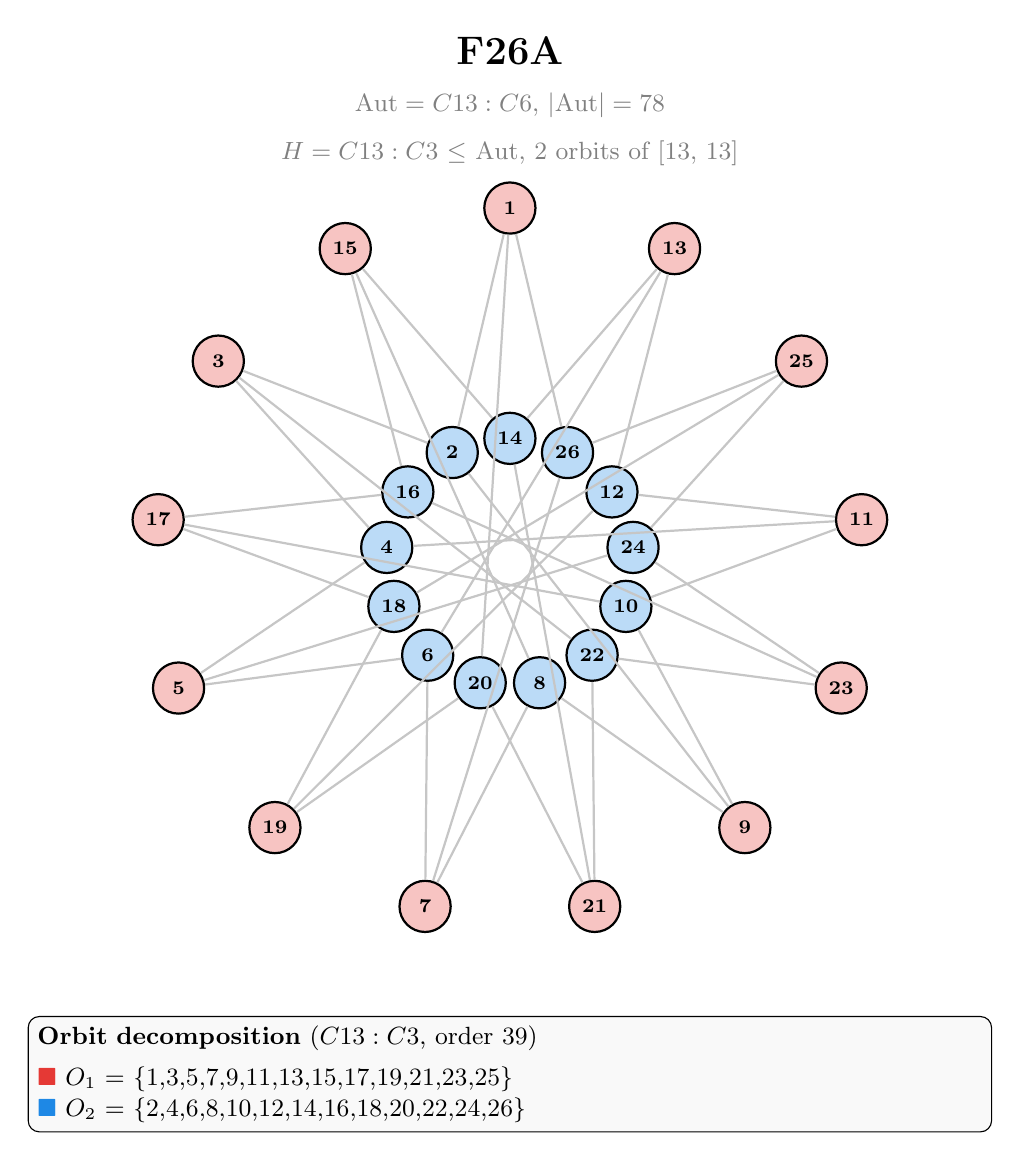
\begin{tikzpicture}[
  vertex/.style={circle, draw, thick, minimum size=6.5mm, inner sep=0pt,
                 font=\scriptsize\bfseries},
  edge/.style={thick, gray!45},
  title/.style={font=\Large\bfseries},
  subtitle/.style={font=\small, text=gray},
]

\node[title] at (0, 6.5) {F26A};
\node[subtitle] at (0, 5.8) {$\mathrm{Aut} = C13 : C6$, $|\mathrm{Aut}| = 78$};
\node[subtitle] at (0, 5.2) {$H = C13 : C3$ $\leq$ $\mathrm{Aut}$, 2 orbits of [13, 13]};

\node[vertex, fill=block0!30] (v1) at (0.000, 4.500) {1};
\node[vertex, fill=block1!30] (v2) at (-0.732, 1.395) {2};
\node[vertex, fill=block0!30] (v3) at (-3.703, 2.556) {3};
\node[vertex, fill=block1!30] (v4) at (-1.564, 0.190) {4};
\node[vertex, fill=block0!30] (v5) at (-4.208, -1.596) {5};
\node[vertex, fill=block1!30] (v6) at (-1.044, -1.179) {6};
\node[vertex, fill=block0!30] (v7) at (-1.077, -4.369) {7};
\node[vertex, fill=block1!30] (v8) at (0.377, -1.529) {8};
\node[vertex, fill=block0!30] (v9) at (2.984, -3.368) {9};
\node[vertex, fill=block1!30] (v10) at (1.473, -0.559) {10};
\node[vertex, fill=block0!30] (v11) at (4.467, 0.542) {11};
\node[vertex, fill=block1!30] (v12) at (1.296, 0.895) {12};
\node[vertex, fill=block0!30] (v13) at (2.091, 3.985) {13};
\node[vertex, fill=block1!30] (v14) at (0.000, 1.575) {14};
\node[vertex, fill=block0!30] (v15) at (-2.091, 3.985) {15};
\node[vertex, fill=block1!30] (v16) at (-1.296, 0.895) {16};
\node[vertex, fill=block0!30] (v17) at (-4.467, 0.542) {17};
\node[vertex, fill=block1!30] (v18) at (-1.473, -0.559) {18};
\node[vertex, fill=block0!30] (v19) at (-2.984, -3.368) {19};
\node[vertex, fill=block1!30] (v20) at (-0.377, -1.529) {20};
\node[vertex, fill=block0!30] (v21) at (1.077, -4.369) {21};
\node[vertex, fill=block1!30] (v22) at (1.044, -1.179) {22};
\node[vertex, fill=block0!30] (v23) at (4.208, -1.596) {23};
\node[vertex, fill=block1!30] (v24) at (1.564, 0.190) {24};
\node[vertex, fill=block0!30] (v25) at (3.703, 2.556) {25};
\node[vertex, fill=block1!30] (v26) at (0.732, 1.395) {26};

\draw[edge] (v1) -- (v2);
\draw[edge] (v1) -- (v20);
\draw[edge] (v1) -- (v26);
\draw[edge] (v2) -- (v3);
\draw[edge] (v2) -- (v9);
\draw[edge] (v3) -- (v4);
\draw[edge] (v3) -- (v22);
\draw[edge] (v4) -- (v5);
\draw[edge] (v4) -- (v11);
\draw[edge] (v5) -- (v6);
\draw[edge] (v5) -- (v24);
\draw[edge] (v6) -- (v7);
\draw[edge] (v6) -- (v13);
\draw[edge] (v7) -- (v8);
\draw[edge] (v7) -- (v26);
\draw[edge] (v8) -- (v9);
\draw[edge] (v8) -- (v15);
\draw[edge] (v9) -- (v10);
\draw[edge] (v10) -- (v11);
\draw[edge] (v10) -- (v17);
\draw[edge] (v11) -- (v12);
\draw[edge] (v12) -- (v13);
\draw[edge] (v12) -- (v19);
\draw[edge] (v13) -- (v14);
\draw[edge] (v14) -- (v15);
\draw[edge] (v14) -- (v21);
\draw[edge] (v15) -- (v16);
\draw[edge] (v16) -- (v17);
\draw[edge] (v16) -- (v23);
\draw[edge] (v17) -- (v18);
\draw[edge] (v18) -- (v19);
\draw[edge] (v18) -- (v25);
\draw[edge] (v19) -- (v20);
\draw[edge] (v20) -- (v21);
\draw[edge] (v21) -- (v22);
\draw[edge] (v22) -- (v23);
\draw[edge] (v23) -- (v24);
\draw[edge] (v24) -- (v25);
\draw[edge] (v25) -- (v26);

\node[draw, rounded corners, fill=gray!5, text width=12cm, align=left, font=\small]
  at (0, -6.5) {
  \textbf{Orbit decomposition} ($C13 : C3$, order 39) \\[4pt]
  \textcolor{block0}{$\blacksquare$} $O_{1}$ = \{1,3,5,7,9,11,13,15,17,19,21,23,25\} \\
  \textcolor{block1}{$\blacksquare$} $O_{2}$ = \{2,4,6,8,10,12,14,16,18,20,22,24,26\}
};

\end{tikzpicture}
\end{document}